\section{Methodology}
\label{sec:methodology}


%%%%%%%%%%%%%%%%%%%%%%%%%%%%%%%%%%%%%%%%%%%stats for old dataset%%%%%%%%%%%%%%%%%%%%%%%%%%%%%%%%%%%%%%%%%%%
\begin{table*}
	\centering
	\caption{Dataset summary} \label{tab-dataset-summary}
	\begin{tabular}{c|c|c|c|c|c|c}%p{0.14\textwidth}
		\hline
		% after \\: \hline or \cline{col1-col2} \cline{col3-col4} ...
		Num. of images crawled & Num. of unique images    & Num. of images downloaded  & Num. of layers downloaded \\
		\hline
		634,412                 & 457,627                 & 346,243                    & 1,763,354  \\
		\hline
		Num. of images analyzed & Num. of layers analyzed & Compressed dataset size              &  Num. of files totally \\
		\hline
		319,620                     & 1,607,533                     & 51TB                        & 117,665,791  \\
		\hline
	\end{tabular}
\end{table*}

%%%%%%%%%%%%%%%%%%%%%%%%%%%%%%%%%%%%%%%%%%%stats for new dataset%%%%%%%%%%%%%%%%%%%%%%%%%%%%%%%%%%%%%%%%%%%
%\begin{table*}
%	\centering
%	\caption{Dataset summary} \label{tab-dataset-summary}
%	\begin{tabular}{c|c|c|c|c|c|c}%p{0.14\textwidth}
%		\hline
%		% after \\: \hline or \cline{col1-col2} \cline{col3-col4} ...
%		Num. of images crawled & Num. of unique images    & Num. of images downloaded  & Num. of layers downloaded \\
%		\hline
%		634,412                 & 457,627                 & 346,243                    & 1,763,354  \\
%		\hline
%		Num. of images analyzed & Num. of layers analyzed & Compressed dataset size              &  Uncompressed dataset size \\
%		\hline
%		344,056                     & 1,748,089                     & 51TB                        & xxx  \\
%		\hline
%	\end{tabular}
%\end{table*}

%\lrcomment{ I think in general it would be good if we emphasize in this section, what
%	was challenging about downloading all this data and how the presented approach
%	overcame these challenges. \nancomment{challenges include: 1. obtaining a list of all the repositories in docker hub; 2. effectively downloading all the images. 3. indept analysis}}

Our methodology consists of three steps~(see Figure~\ref{fig-downloader-analyzer}):
i)~crawl Docker Hub to list all repositories;
ii)~download the latest image (and referenced layers) from each repository based
on the crawler results; iii) unpack and analyze images and layers.


\begin{figure}
	\centering
	% Requires \usepackage{graphicx}
	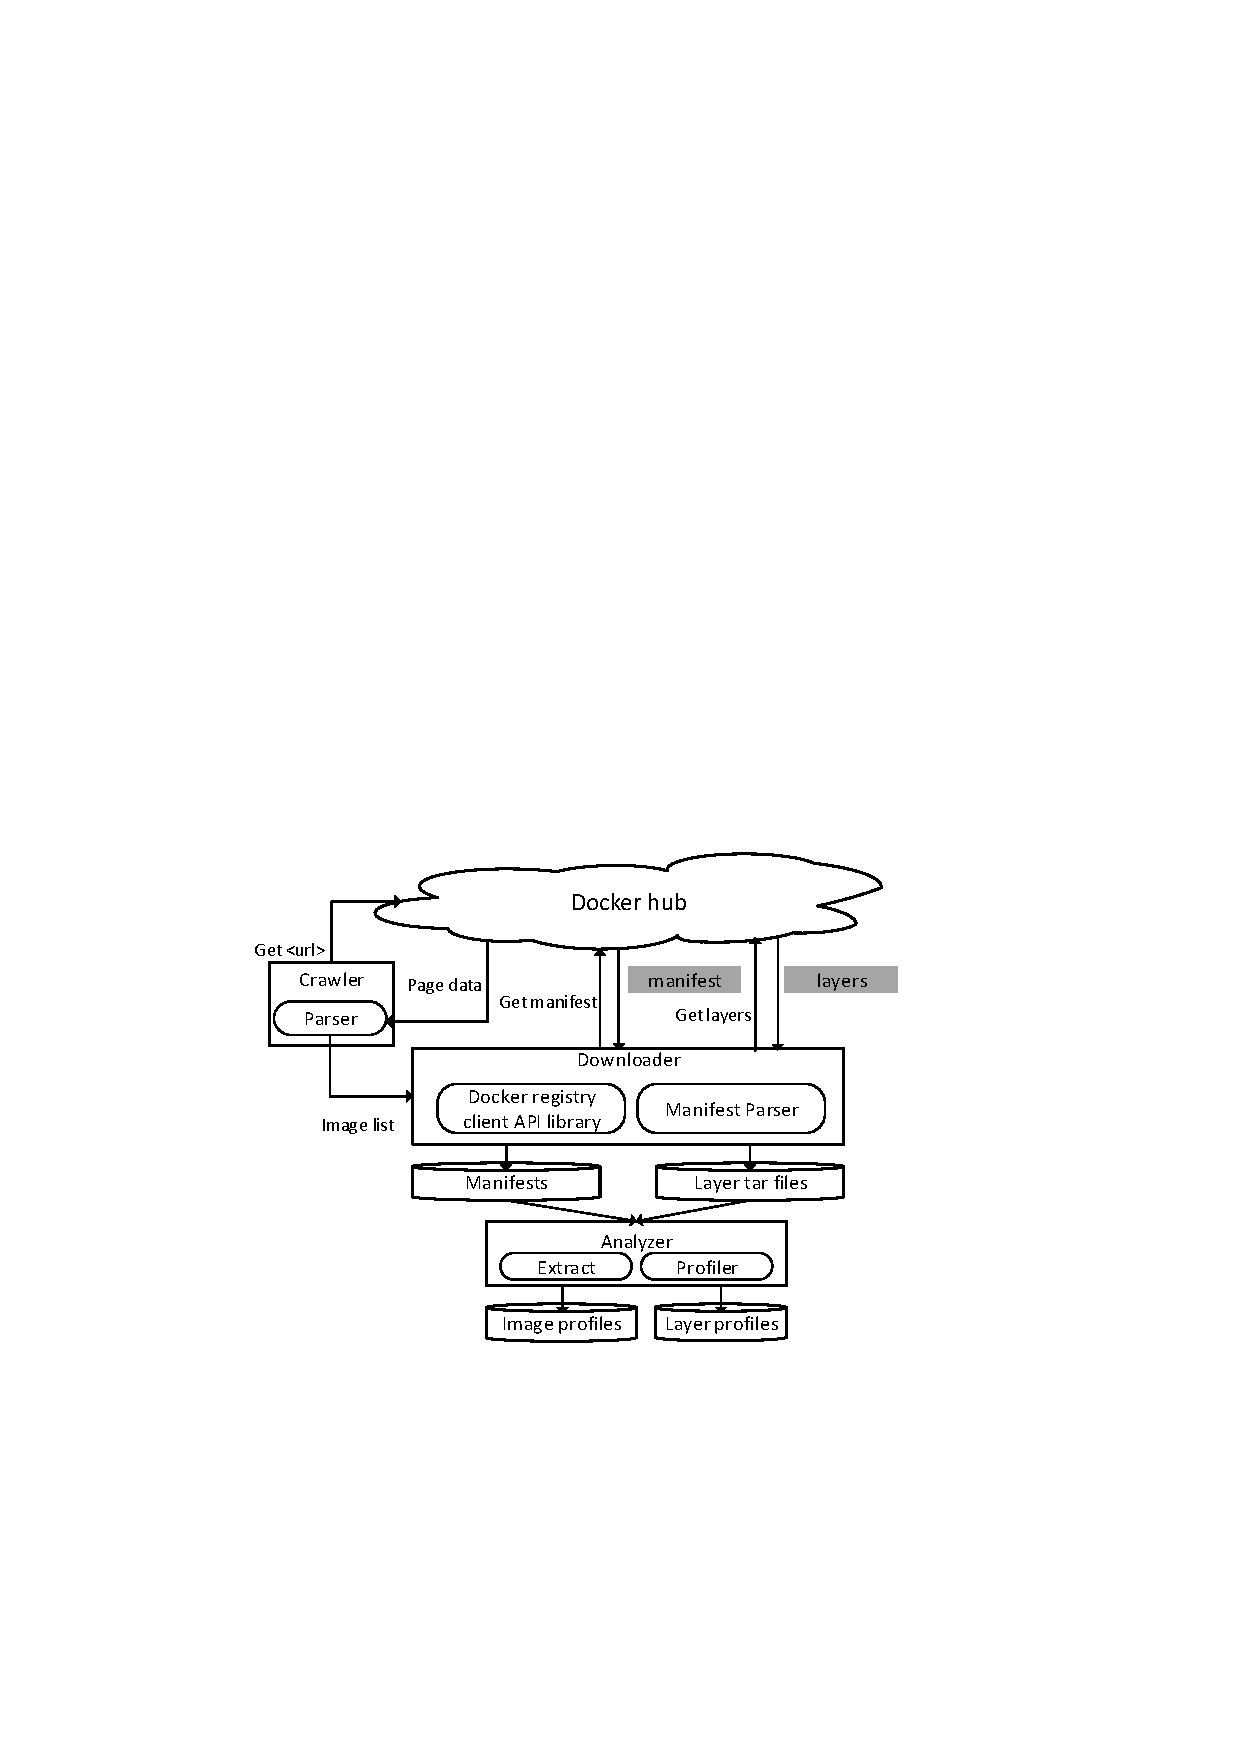
\includegraphics[width=0.5\textwidth]{graphs/fig-downloader-analyzer.pdf}\\
	\caption{Crawler, Downloader, and Analyzer
		%\vcomment{Can we add colors to this figure? Also, increase the font a bit.}
	}
	\label{fig-downloader-analyzer}
\end{figure}

\subsection{Crawler}
\label{sec:crawler}

% TODO: The following paragraph seems out of place (move to next subsection?).

To download a particular image, %or set of images (i.e., a repository)
the name of the repository name which the image belongs to needs to be provided.
The crawler is responsible for generating a list of repositories for the downloader.

Public repositories 
in Docker Hub
(i.e., the repositories
that anyone can pull from)
re divided into official
repositories---served by the Docker Hub partners---and non-official
repositories---provided by regular users and third-party organizations.
%
The number official repositories is less than 200, while, the majority
of repositories in Docker Hub are non-official (over 400 thousand).
Listing non-official repositories requires web crawling because
Docker Hub does not provide an API to retrieve all repository names.
%Therefore, we implemented a Crawler to crawl Docker Hub and list all non-official
%repositories.

Our crawler utilizes the Docker Hub search engine to find all available
repositories.
%
As the name of non-official repositories is comprised
of the user name and the repository name separated by a ``/'', %as detailed in \ref{sec:docker-registry},
we can search for ``/'' and obtain a list of all non-official repositories.
The Crawler downloads all pages from the search results and parses the web content
to build a list of all non-official repositories.
We ran the crawler on May 30th, 2017 and it delivered a list of 634,412 repositories.
%
%However, the obtained list contained duplicate entries because 
%the crawling process is not atomic and some repositories have ``/'' in their description.
%
After removing duplicate entries (introduced by Docker Hub indexing logic),
the final repository list consists of 457,627
distinct repositories. 
% TODO: Could we mention something about this number difference? Readers will immediately wonder.

\subsection{Downloader}
\label{sec:downloader}

%Docker repository is a set of images labeled with \emph{version tags}.
Images in Docker Hub repositories are labeled with \emph{version tags}
to track different image versions.
%The different images in the repository are labeled with tags.
%
%For example, \texttt{ubuntu:17.10} refers to image version \texttt{17.10} in the
%\texttt{ubuntu} repository.
%
If no tag is provided when pulling an image, 
Docker pulls the \texttt{latest} tag by default.
%For example, \texttt{docker pull ubuntu} command pulls the
%\texttt{ubuntu:latest} image.
%
In this work we focus on downloading images with the \texttt{latest} tag to
make the analysis more feasible. We believe that the latest
image versions represent the most up-to-date state of the images.
%
%and plan to analyze images with other tags in the future.

Instead of using the Docker client to download images,
we implement our own downloader, which calls the Docker registry API
directly~\cite{dockerregistryclient} to download manifests
and image layers in parallel.
%We use Docker registry client library~\cite{dockerregistryclient} to simultaneously
%download manifests and image layers.
%\lrcomment{What does `original' mean here? \nancomment{without any modification}}
%
Our downloader runs significantly faster than a \texttt{docker pull}-based downloader
because the latter one performs operations besides downloading the image.
For example, it automatically extracts each layer's tar archive file
and creates the corresponding read-only snapshot using the configured
Docker storage driver.
This not only takes considerable amount of time but also leads
to overly high storage space utilization.
%
Furthermore, the local storage format of Docker client makes it difficult
to analyze the contents of each layer separately.
% TODO: Why is it difficult? (we're making a claim)
%
% TODO: The following sentence is mostly repetition of start of paragraph.
Our downloader can download multiple images simultaneously and fetch
the individual layers of an image in parallel. Layers are transferred as gzip
compressed tar archives.

%The process consists of two steps.
%
%First, fetching the manifest by sending a \texttt{GET} request to
%$/v2/\langle name \rangle/manifests/\langle reference \rangle$,
%where~\textit{name} refers to
%$\langle namespace\rangle/\langle repository name \rangle$
%and \textit{reference} is typically a version $\langle tag \rangle$.
%
%Second, once the manifest is downloaded, the downloader uses the layer digests to
%download individual layers
%%(including the config file for Schema 2 versioned manifest)
%by sending $GET$ request to $/v2/\langle name \rangle/blobs/\langle digest \rangle$.
%\textit{Name}, as for manifests,
%refers to $\langle namespace\rangle/\langle repository name \rangle$
%while~\textit{digest} refers to the layer digest.
%Layers are transferred as gzip compressed tar archives.

The whole downloading process took around 30 days.
%
Overall, we downloaded 51~TB of data in 355,319 image manifests with 1,792,609
compressed layers.
%
A total of 111,384 images could not be downloaded due to three reasons:
%
1)~5\% of these images required authentication;
2)~87\% of these images did not have a \texttt{latest} tag; and
3)~8\% of these images contained layers that cannot be downloaded.
% 0.05189255189	0.8666056166 0.0815018315
%As we discussed in Section~\ref{sec:crawler}, we only downloaded the \texttt{latest}
%version of an image to shorten the downloading process.
Table~\ref{tab-dataset-summary} summarizes the properties of the downloaded
dataset.


\subsection{Analyzer}
\label{sec:analyzer}

The analyzer extracts the downloaded layers
and analyzes them along with the image manifests.
For each image, it creates an image profile and individual layer profiles,
which contain metrics for the whole image and
its individual layers, respectively.
%Profiles are stored in JSON format.

\paragraph{Layer profile}

%Layers are downloaded as compressed tar archive files.
%
To produce the layer profile, the analyzer first decompresses and extracts each
layer tarball to a layer directory.
%
Then, it recursively traverses each subdirectory and obtains
its metadata information. Note that 8.8\% of the layers reported errors during
extraction and could not be analyzed.
%that we analyzed 91.2\% of 
%the layers we downloaded. The rest 8.8\% of layers have errors during extracting.
%\lrcomment{put reason here}\nancomment{addressed}
%Note that we excluded the compressed layer
%archives that are bigger than 2 GB from the analysis because \lrcomment{put reason here}.
%These comprise only a small subset of 1,268 layers.
%
A layer profile consists of:
%\nancomment{could remove archival size}
\begin{compactenumerate}
\item Layer metadata: \{
layer digest; 
%archived layer size (ALS); 
sum of contained file sizes (FLS); 
compressed layer size (CLS); 
directory count;
file count;
max. directory depth
%\lrcomment{How is this different from directory depth below?}\nancomment{addressed};
\}

\item Compression ratio: \{
%ALS-to-CLS;
FSL-to-CLS;
\}

\item Directory metadata (for every directory in the layer): \{
directory name;
directory depth;
file count;
directory size;
\}

\item File metadata (for every file in the layer): \{
file name;
file digest;
file type;
file size;
\}
\end{compactenumerate}
%\vcomment{Instead of the table, let's us the itemized list above for now,
%\nancomment{already add table 1. and we dont need to list metrics here since we present
%them in results}}


\paragraph{Image profile}

To create the image profile, the analyzer parses the manifest
and obtains the configuration information such as OS and target architecture.
Further, once individual layers are analyzed, the analyzer builds the image
profile by including pointers to its layer profiles. An image profile consists of:
\begin{compactenumerate}

\item Image metadata: \{
image name; 
%archived image size (AIS); 
sum of containing file sizes (FIS); 
compressed image size (CIS); 
Directory count;
File count;
\}

\item Compression ratio: \{
%AIS-to-CIS;
FIS-to-CIS;
\}

\end{compactenumerate}

We released both the software that we designed
to download the images and all profiles we generated
publicly at {\small{\url{https://elided.for.review}}}.

%%%%%%%%%%%%%%%%%%%%%%%%%%%%%%%%%%%%%%%%%%%%%%%%%%%%%%%%%%%%%%%%%%%%%%%%%%%%%%
%                                                                            %
%                                OLD METHO                                   %
%                                                                            %
%%%%%%%%%%%%%%%%%%%%%%%%%%%%%%%%%%%%%%%%%%%%%%%%%%%%%%%%%%%%%%%%%%%%%%%%%%%%%%
%%\nancomment{
%%	TODO: \\
%%	1. Complete fig and table\\
%%}
%
%\lrcomment{ I think in general it would be good if we emphasize in this section, what
%was challenging about downloading all this data and how the presented approach
%overcame these challenges. \nancomment{challenges include: 1. obtaining a list of all the repositories in docker hub; 2. effectively downloading all the images. 3. indept analysis}}
%
%Our methodology consists of three steps~(Figure~\ref{fig-downloader-analyzer}):
%1)~crawl Docker Hub to list all official and nonofficial repositories;
%2)~download the latest image (and referenced layers) from each repository based
%on the crawler results; 3) unpack and analyze images and layers.
%
%%
%%
%%The first step is to massively download the Docker images from Docker registry.
%%
%%When the images are downloaded, we analyze them and calculate statistics distribution for
%%different metrics.
%%
%%The details of each step are covered in the following sections.
%%
%%\vcomment{I suggest to restructure this section simirarly to background to
%%revolve around the figure. Once you add the diagram describing our methodology
%%(like we put on the whiteboard ones), start describing components on it in the
%%order they are used: crawler, downloader, analyzer. Having two subsection:
%%``downloader'' and ``downloading images'' is confusing.
%%
%%We might want to have less deep structure also:
%%
%%3. Methodology
%%  (Figure)
%%3.1 Crawler
%%3.2 Downloader
%%3.3 Analyzer
%%}
%%
%%\nancomment{addressed}
%
%%\nancomment{
%%	figures are stored in google drive, the link is pinned in slacker;
%%	%https://drive.google.com/open?id=0B4jePsYXW6SSTTRLb0FHVXVjNUk
%%	figures/fig-docker-architecture.pdf}\\
%
%
\begin{figure}
	\centering
	% Requires \usepackage{graphicx}
	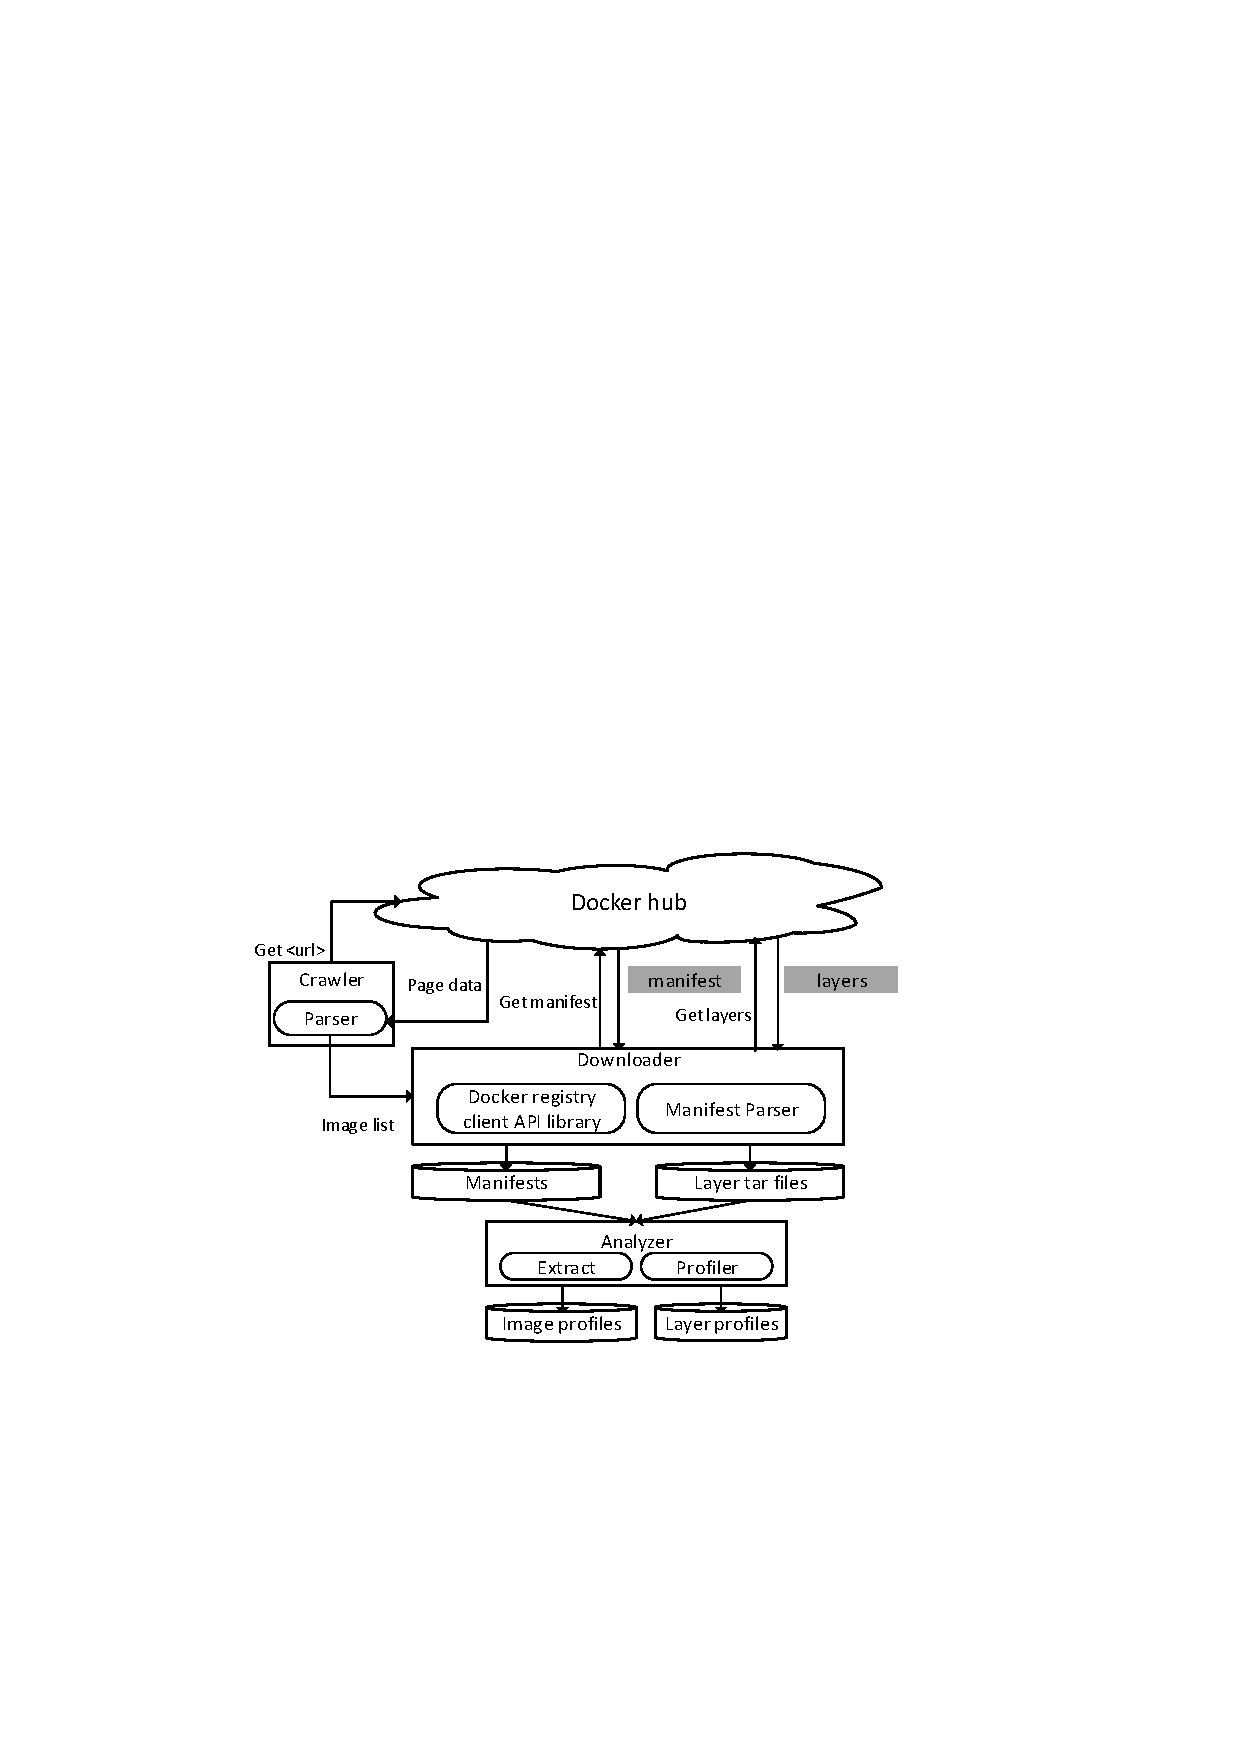
\includegraphics[width=0.5\textwidth]{graphs/fig-downloader-analyzer.pdf}\\
	\caption{Crawler, Downloader, and Analyzer
		%\vcomment{Can we add colors to this figure? Also, increase the font a bit.}
	}
	\label{fig-downloader-analyzer}
\end{figure}
%
%%how container deameon.
%%
%\subsection{Crawler}
%\label{sec:crawler}
%
%%
%To download a particular image, %or set of images (i.e., a repository)
%the name of the repository name which the image belongs to should be provided.
%The crawler is responsible
%for generating a list of repositories for the downloader.
%%as mentioned in Section~\ref{sec:docker-registry}. 
%%
%%
%%
%%\vcomment{Here and in the whole text we need to be very carefull distinguishing names 
%%of repository and image. Also discussion on image tags is missing, should be in
%%background section.}
%%\nancomment{addressed.}
%%
%Public repositories in Docker registry are divided into official
%repositories---served by the Docker Hub's partners---and non-official
%repositories---provided
%by regular users and third-party organizations.
%%, where For example, official repository Ubuntu Here is an example of the shared 
%%repository official repository Ubuntu and one of its tags. 
%%
%%A repository is a set of Docker images. A repository can be shared by pushing it to a
%%registry server. 
%%Public repositories in Docker registry can be divided into official images and non-official 
%%images.
%%
%The number official repositories is less than 200,
%% The list of official repositories
%%can be retrieved via \lrcomment{add how to list official repos}
%while, the majority
%of repositories in Docker Hub (about 400 thousands)
%are non-official.
%% (around \lrcomment{add number}).
%Listing non-official repositories requires web crawling because
%%to the best of our knowledge,
%Docker Hub does not provide an API to retrieve all repository names.
%
%Therefore, we implemented a Crawler to crawl Docker Hub and list all non-official
%repositories.
%%
%Docker Hub provides a search engine which indexes public repositories and allows
%users to search for a repository according to
%some search string. 
%%
%As the name of non-official repositories is comprised
%of the user name and the repository name separated by a ``/'',
%we can search for ``/'' and obtain a list of all non-official
%repositories.
%%``$\langle namespace\rangle/\langle repository name \rangle $", where~\textit{namespace}
%%is the user name. 
%%
%%In this case, we search for `/' and obtain a list of repositories which contains '/'.
%%
%%In other words, this method lists all the non-official public repositories in Docker Hub.
%%
%The Crawler downloads all pages from the search result.
%%
%Once web pages are downloaded, it parses the web content to build a list of
%all non-official repositories.
%
%%\lrcomment{It may be good to discuss how accurate this method is. Can we miss anything?
%%Can we get wrong results?}
%
%
%
%We ran the crawler on May 30th, 2017 and it delivered a list of 634,412 repositories.
%%
%However, the obtained list contained duplicate entries because 
%the crawling process is not atomic and some repositories have ``/'' in their description.
%%
%After removing all duplicates, the final repository list consists of 457,627
%distinct repositories. 
%%
%
%
%%
%%\vcomment{Explain why, state that it is future work.} 
%%\nancomment{addressed}
%%
%%\vcomment{I'd comment out discussion on '*'---it has low importance.}
%%\nancomment{addressed. let's comment it now and see how to deal with this issue}
%%Note that the namespace of official images is `\textit{library}'.
%%
%
%\subsection{Downloader}
%\label{sec:downloader}
%
%Docker repository is a set of images labeled with \emph{version tags}.
%%The different images in the repository are labeled with tags.
%%
%For example, \texttt{ubuntu:17.10} refers to image version \texttt{17.10} in the
%\texttt{ubuntu} repository.
%%
%If user does not provide a tag when pulling an image, 
%Docker daemon uses the \texttt{:latest} tag by default.
%For example, \texttt{docker pull ubuntu} command pulls the
%\texttt{ubuntu:latest} image.
%%
%In this work we only download images with the \texttt{:latest} tag to
%make the analysis more feasible.  We believe that the latest
%images versions represent most up-to-date state of  Docker images
%%
%and plan to analyze images with other tags in the future.
%
%
%
%%The downloader takes the list from the crawler as an input and retrieves
%%all the listed images from Docker Hub (see Figure~\ref{fig-downloader-analyzer}).
%%
%Instead of using Docker CLI to download images,
%%via the Docker Engine,
%we wrote our own downloader that calls Docker registry API directly.
%We used Docker registry client~\vcomment{insert the name, \nancomment{it is called Docker registry client}} library~\cite{dockerregistryclient} to simultaneously
%download \emph{original} manifests and image layers. \lrcomment{What does
%`original' mean here? \nancomment{without any modification}}
%%
%%\vcomment{Should we mention and cite the library that we used here?}
%%
%%\nancomment{addressed (cited in the following para)}
%%
%%
%%We decided to implement a separate downloader due to several reasons:
%%
%Our downloader runs significantly
%faster than \texttt{docker pull}-based downloader
%because the latter one performs
%operations other than downloading the
%image.
%%such as extracting
%%tar archive files and converting manifest version. 
%%
%For example, it automatically extracts each layer's tar archive file
%and creates corresponding read-only snapshot with  configured Docker storage driver.
%%and converts the manifests that are schema version 1 to schema version 2
%%(starting from Docker engine version 1.10).
%This
%not only takes considerable amount of time but also leads
%to overly high storage space utilization.
%%
%% affects
%%our results about manifest version statistics;
%%
%Furthermore, the local storage format of Docker client makes it difficult
%to analyze the contents of each layer separately.
%%Second, layer content directories are not visible for some Docker storage
%%drivers, e.g., devicemapper, which is not feasible to analyze the layer
%%content. 
%%
%%\vcomment{I think most importantly it is faster because we do not need to
%%perform extra steps that Docker client performs.}
%%\nancomment{addressed}
%%
%
%Our downloader can download multiple images simultaneously and fetch
%the individual layers of an image in parallel.
%%within each image downloading process, layers are downloaded in parallel.
%%
%%To download the original manifests and layers from Docker Hub, downloader
%%embeds a library called Docker registry client API citeXXX which only encapsulates
%%manifest and layer downloading functions in Docker engine without extracting layer
%%tarball and converting manifest version. 
%%
%%
%%\subsubsection{Downloading images}
%%
%%\vcomment{definitely need to merge this subsection with Downloader subsection.
%%See my comment for the whole section.}
%%\nancomment{addressed}
%%
%%As shown in Figure~\ref{fig-downloader-analyzer}, downloader first obtains a 
%%list of public images through crawling Docker Hub.
%%
%%Then, it starts downloading process.
%%
%%It mainly downloads two components: manifest and individual layer files. 
%The process consists of two steps.
%%
%First, fetching the manifest by sending a \texttt{GET} request to
%$/v2/\langle name \rangle/manifests/\langle reference \rangle$,
%where~\textit{name} refers to
%$\langle namespace\rangle/\langle repository name \rangle$
%and \textit{reference} is typically a version $\langle tag \rangle$.
%%
%%
%%\lrcomment{Are the following 4 sentences needed?}
%%Note that the~\textit{namespace} of official is~\textit{library}.
%%
%%The reference can include a tag or digest.
%%
%%Note that currently we only downloaded the images with~\textit{latest} tag to shorten
%%the downloading process. In the future, we will download all the images with different tags.
%%
%%As discussed in Section~\ref{xxx}, manifest consist of multiple layer digests.
%%
%%Note that Schema 2 versioned manifest also contains a config file digest.
%%\vcomment{I believe we never explained what is config file. We need to discuss in
%%in background section.}
%%\lrcomment{Do we use config files in the analysis? If they contain the command
%%to run in the container, I think that could give us some interesting insights into
%%how people use containers.}
%%
%Second, once the manifest is downloaded, the downloader uses the layer digests to
%download individual layers
%%(including the config file for Schema 2 versioned manifest)
%by sending $GET$ request to $/v2/\langle name \rangle/blobs/\langle digest \rangle$.
%\textit{Name}, as for manifests,
%refers to $\langle namespace\rangle/\langle repository name \rangle$
%while~\textit{digest} refers to the layer digest.
%%or config file digest.
%Layers are transferred as gzip compressed tar archives.
%%\vcomment{What compression is used?}
%%\nancomment{addressed}
%
%%
%%\vcomment{I believe different parts of this section belong to different
%%	earlier parts: some to crawler, some to downloader.}
%%\nancomment{addressed}
%%
%
%
%The whole downloading process took around 30 days.
%%
%Overall, we downloaded 51~TB of data in 355,319 image manifests with 1,792,609
%compressed layers.
%%
%A total of 111,384 images could not be downloaded due to three reasons.
%%
%First, 5\% of the images required authentication and
%second, 87\% of the images did not have the \texttt{latest} tag.
%Third, 8\% of the images contains layers that cannot be downloaded.
%% 0.05189255189	0.8666056166 0.0815018315
%%As we discussed in Section~\ref{sec:crawler}, we only downloaded the \texttt{latest}
%%version of an image to shorten the downloading process.
%Table~\ref{tab-dataset-summary} summarizes the properties of downloaded
%dataset.
%
%%\nancomment{2. TODO: add a table discribe:\\
%%	how many images, duplicate ratio\\
%%	how many cannot download, (removed, no latest)\\
%%	how many layers, config, manifest\\
%%	dataset}
%
%%\subsubsection{Docker image dataset statistics}
%
%
%
%%The reason probably is that Docker Hub adjusted websites'order or modified the
%%websites because of the increasing of Docker images during our crawling process.
%%Our crawler has a unavoidable delay between each HTTP requst and HTTP response. 
%%So it couldn't reflect the websites'order or website content changes. Another
%%reason is that search engine lists duplicated images 
%
%%Overall, we downloaded XXX image with XXX layers. Table~\ref{XXX} summaries
%%the statistics of Docker image dataset we downloaded. Then, we profiled the
%%layers, config files, and manifests we downloaded and calculated the statistic
%%distribution for different metrics. 
%
%%Some embedded literal typset code might 
%%look like the following :
%%
%%{\tt \small
%%\begin{verbatim}
%%int wrap_fact(ClientData clientData,
%%              Tcl_Interp *interp,
%%              int argc, char *argv[]) {
%%    int result;
%%    int arg0;
%%    if (argc != 2) {
%%        interp->result = "wrong # args";
%%        return TCL_ERROR;
%%    }
%%    arg0 = atoi(argv[1]);
%%    result = fact(arg0);
%%    sprintf(interp->result,"%d",result);
%%    return TCL_OK;
%%}
%%\end{verbatim}
%%}
%%
%%Now we're going to cite somebody.  Watch for the cite tag.
%%Here it comes~\cite{Chaum1981,Diffie1976}.  The tilde character (\~{})
%%in the source means a non-breaking space.  This way, your reference will
%%always be attached to the word that preceded it, instead of going to the
%%next line.
%
%\begin{table*}
%	\centering
%	\caption{Dataset summary} \label{tab-dataset-summary}
%	\begin{tabular}{c|c|c|c|c|c|c}%p{0.14\textwidth}
%		\hline
%		% after \\: \hline or \cline{col1-col2} \cline{col3-col4} ...
%		Num. of images crawled & Num. of unique images    & Num. of images downloaded  & Num. of layers downloaded \\
%		\hline
%		634,412                 & 457,627                 & 346,243                    & 1,763,354  \\
%		\hline
%		Num. of images analyzed & Num. of layers analyzed & Compressed dataset size              &  Uncompressed dataset size \\
%		\hline
%		344,056                     & 1,748,089                     & 51TB                        & xxx  \\
%		\hline
%	\end{tabular}
%\end{table*}
%
%\subsection{Analyzer}
%\label{sec:analyzer}
%
%The analyzer analyzes extracts downloaded layers
%and analyzes them along with image manifests.
%It creates two types of profiles for each image:
%an image profile and individual layer profiles.
%Each profile contains different metrics for the whole image and
%its individual layers, respectively.
%Profiles are stored in JSON format.
%
%
%%
%%\vcomment{I think we do not need to discuss any metrics above, as you
%%discuss them below in corresponding subsections.}
%%\nancomment{addressed}
%%
%
%\paragraph{Layer profile.}
%
%Layers are downloaded as compressed tar archive files.
%%
%To produce the layer profile, the analyzer first decompresses and extracts each
%layer tarball to a layer directory.
%%
%Then, it recursively traverses each subdirectory and obtains
%the metadata information for each subdirectory.
%
%The layer profile contains metadata about the layer, its directories,
%and files: 
%
%\{
%layer digest; 
%Archived layer size (ALS); 
%Sum of containing file sizes (FLS); 
%Compressed layer size (CLS); 
%ALS-to-CLS (compression ratio);
%FSL-to-CLS (compression ratio);
%Directory count;
%File count;
%Layer directory depth;
%\}
%
%\{
%Directory name;
%Directory depth;
%File count;
%Directory size;
%\}
%
%\{
%File name;
%File digest;
%File type;
%File size;
%\}
%
%\begin{compactitemize}
%	\item XXX
%	\item XXX
%	\item XXX
%	\item XXX
%\end{compactitemize}
%
%%file count while directory metadata covers directory depth and size
%%and file metadata includes size and type. The full set of metrics
%%covered by the layer profile is shown in Table~\ref{xxx}.
%
%
%%Each layer profile contains
%%layer metadata information, such as layer size and file count; and
%%directory metadata information for each subdirectory, such as directory
%%depth and directory size; and file metadata information for each file,
%%such as file size and file type.
%%
%%\vcomment{I'm not sure what figure we want here. I think a table might suffice.}
%%\nancomment{addressed}
%%\nancomment{3. TODO: 
%%	add a fig: discribe all layer metadata, config metadata, and manifest metadata structure} 
%%
%%\nancomment{4. TODO: 
%%	add a table\\
%%	layer tarball format statistics, tar, compressed, non compressed\\
%%	config statistics, txt, json\\
%%	manifest statistics, txt, json}
%\vcomment{Instead of the table, let's us the itemized list above for now, \nancomment{already add table 1. and we dont need to list metrics here since we present them in results}}
%
%
%\paragraph{Image profile.}
%
%To create the image profile, the analyzer parses the manifest
%and obtains the configuration information such as OS and architecture.
%Further, once individual layers are analyzed, the analyzer can build the whole image
%profile by including pointers to its layer profiles. In total, image profile includes
%the following information:
%\{
%Image name; 
%Archived Image size (AIS); 
%Sum of containing file sizes (FIS); 
%Compressed image size (CIS); 
%ALS-to-CLS (compression ratio);
%FSL-to-CLS (compression ratio);
%Directory count;
%File count;
%\}
%
%\begin{compactitemize}
%	\item XXX
%	\item XXX
%	\item XXX
%	\item XXX
%\end{compactitemize}
%
%% image metadata information,
%%such as image pull count and layer count, and image configuration
%%information, such as OS version and architecture. All metrics
%%in the image profile are shown in Table~\ref{xxx}.
%
%%Note that schema version 2 manifests store configuration information in a
%%config file as discussed in Section~\ref{sec-image-layers}.
%%\lrcomment{I think we removed the part about different manifest versions from
%%the background, should add it back.}
%%
%%As shown in table~\ref{xxx}, \gap of manifests are Schema version 2 while the
%%rest are Schema version 1. 
%
%%
%%
%%While layer profile
%%contains layer metadata information, such as layer size and file count;
%%and directory metadata information for each subdirectory, such as directory
%%depth and directory size; and file metadata information for each file, such
%%as file size and file type.
%%
%%Table~\ref{xxx} summaries the layer archive file, config file, and manifest
%%statistics.
%
%
%%\vcomment{This section (and some other places) contain a lot of ``etc.''. The
%%general rul of thumb never to ue etc. in a scientific paper. Instead,
%%say: "e.g.,", or "for example," or "for instance"}
%%\nancomment{addressed}
%%\subsubsection{Config profile}
%
